% ============================================================================
%  expl1.tex -- generated by pipeline/5_results/kb_explanation.py -- do not edit by hand
%
%  One panel of the worked example for job 3031 x cv 447 (see the module docstring).
%  All labels, counts and scores are read from the ESCO v1.2.1 graph.
%
%  Compile: pdflatex expl1.tex        (needs TikZ, no extra fonts)
% ============================================================================
\documentclass[border=4pt]{standalone}
\usepackage{tikz}
\usepackage[T1]{fontenc}
\usepackage{amsmath}
\renewcommand{\familydefault}{\sfdefault}
\usetikzlibrary{arrows.meta,positioning,backgrounds,calc}

% --- palette shared with example_esco.tex ----------------------------------
\definecolor{occLeaf}{HTML}{FCE3C1}
\definecolor{skLeaf}{HTML}{CFE6F7}
\definecolor{skGrp}{HTML}{9FC9E8}
\definecolor{shared}{HTML}{E8617A}
\definecolor{faraway}{HTML}{999999}

\begin{document}
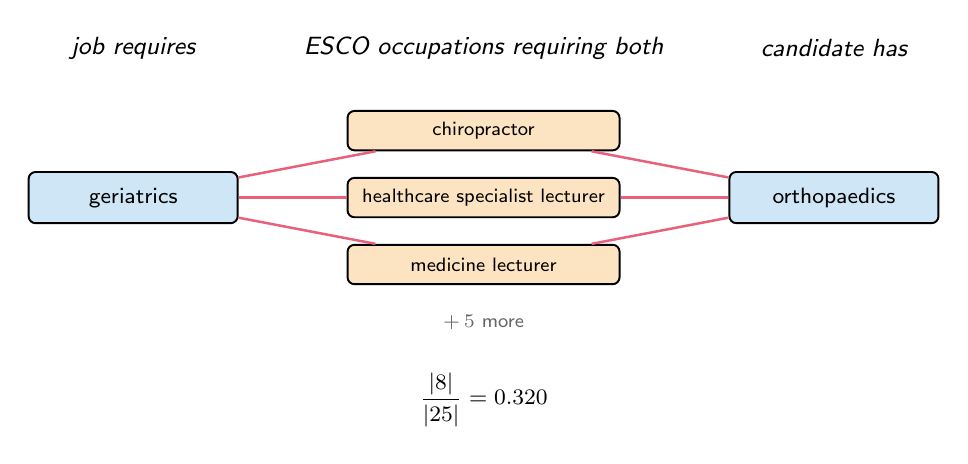
\begin{tikzpicture}[
  font=\footnotesize,
  node/.style={draw=black,line width=0.7pt,rounded corners=2.5pt,align=center,
               text width=25mm,inner sep=2.2pt,minimum height=6.5mm},
  skL/.style={node,fill=skLeaf},
  skG/.style={node,fill=skGrp,text width=26mm},
  occN/.style={node,fill=occLeaf,text width=33mm,minimum height=5mm,font=\scriptsize},
  occDead/.style={occN,fill=occLeaf!35,draw=black!45,densely dashed},
  bridge/.style={draw=shared,line width=0.9pt},
  dead/.style={draw=black!35,line width=0.7pt,densely dotted},
  broader/.style={densely dashed,draw=black!55,line width=0.8pt},
  near/.style={draw=shared,line width=1.5pt},
  detour/.style={draw=faraway!45,line width=3.4pt,line cap=round,line join=round},
  score/.style={align=center,font=\footnotesize},
  more/.style={align=center,font=\scriptsize,text=black!60},
  cross/.style={font=\normalsize,text=faraway},
  hdr/.style={font=\small\itshape,anchor=center},
]
  \node[hdr] at (0.0,1.90) {job requires};
  \node[hdr] at (4.45,1.90) {ESCO occupations requiring both};
  \node[hdr] at (8.9,1.90) {candidate has};
  \node[skL] (jl) at (0.0,0) {geriatrics};
  \node[skL] (cl) at (8.9,0) {orthopaedics};
  \node[occN] (o0) at (4.45,0.85) {chiropractor};
  \draw[bridge] (jl) -- (o0);
  \draw[bridge] (o0) -- (cl);
  \node[occN] (o1) at (4.45,0.00) {healthcare specialist lecturer};
  \draw[bridge] (jl) -- (o1);
  \draw[bridge] (o1) -- (cl);
  \node[occN] (o2) at (4.45,-0.85) {medicine lecturer};
  \draw[bridge] (jl) -- (o2);
  \draw[bridge] (o2) -- (cl);
  \node[more,below=2.5mm of o2] (more) {$+\,5$ more};
  \node[score,below=3mm of more] {$\dfrac{|8|}{|25|} = 0.320$};
\end{tikzpicture}
\end{document}
